With dates for \DiachronicPassages{} passages, the corpus can be asked whether
it shows the story the period is usually told as: the moral sense of Hutcheson
giving way to sympathy, and sympathy in turn to the calculating language of
utility and interest. We count the share of passages in each quarter-century
that use each term --- rates, not counts, since the corpus is wildly uneven
across time and raw counts would only redraw Figure~\ref{fig:corpus}.

\begin{figure}[t]
  \centering
  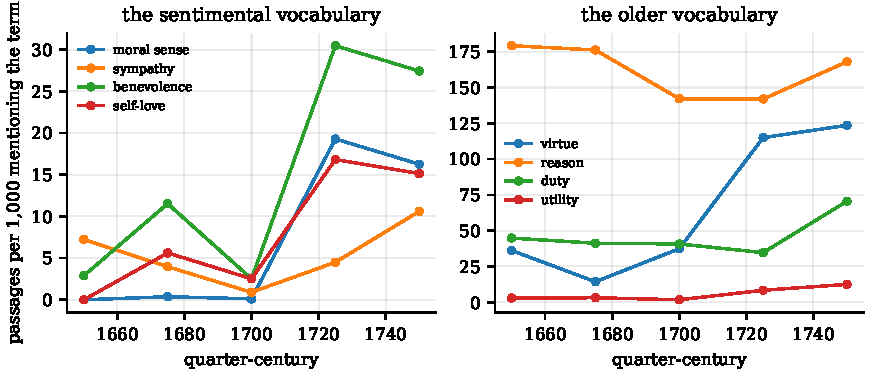
\includegraphics[width=\linewidth]{diachrony.pdf}
  \caption{Term use per 1,000 dated passages by quarter-century. Left: the
           vocabulary of moral sentiment, absent before 1700 and arriving
           together. Right: the older vocabulary, present throughout.}
  \label{fig:diachrony}
\end{figure}

The first half of the story is visibly there, and sharply. \emph{Moral sense}
does not occur at all in the first two bins --- a rate of \FirstMoralSense{}
per thousand --- and peaks in the bin beginning \PeakMoralSense{} at
\PeakRateMoralSense{}. \emph{Self-love} does the same thing on the same
schedule, from \FirstSelfLove{} to a peak of \PeakRateSelfLove{}, and
\emph{benevolence} rises from \FirstBenevolence{} to \PeakRateBenevolence{}.
These three arrive together, in the quarter-century that contains Hutcheson's
\emph{Inquiry} and \emph{Essay} \citep{hutcheson1725,hutcheson1728} and
Butler's \emph{Sermons} \citep{butler1726}. A vocabulary appears from nothing
and takes over a literature inside twenty-five years.

The second half of the story is not there, at least not here.
\emph{Sympathy} rises only modestly, from \FirstSympathy{} to
\LastSympathy{}, and never approaches the prominence of the moral-sense
cluster. \emph{Utility} likewise ends at \LastUtility{}. The obvious
explanation is the corpus rather than the period: it thins after 1750, and the
works that would carry the sympathy story --- Hume's \emph{Treatise}
\citep{hume1740} and Smith's \emph{Theory of Moral Sentiments}
\citep{smith1759} --- are represented thinly, a gap the retrieval agent
discovered independently and reported unprompted when asked to compare the two
(\S\ref{sec:limits}).

The unglamorous terms are the ones that dominate throughout. \emph{Reason}
runs at \FirstReason{} per thousand in the earliest bin and
\LastReason{} in the latest, an order of magnitude above anything in the
sentimental cluster, and declines only gently. \emph{Virtue} more than
triples, from \FirstVirtue{} to \LastVirtue{}. \emph{Obligation} and
\emph{duty} both rise substantially. Whatever else happened to British moral
philosophy across this period, the words it spent most of its time using were
not the ones it is remembered for introducing --- a result consistent with
what \S\ref{sec:graph} found in the map's hubs, arrived at by a completely
different route.
